\documentclass{article}
\usepackage[margin=0.65in]{geometry}
\usepackage{enumitem}
\usepackage{graphicx}
\usepackage{hyperref}
\usepackage{titlesec}
\usepackage{xcolor}
\hypersetup{hidelinks}
\setlist[itemize]{leftmargin=1.5em,topsep=2pt,itemsep=1pt,parsep=0pt,partopsep=0pt}
\titlespacing*{\section}{0pt}{1.2ex}{0.6ex}
\setlength{\parindent}{0pt}
\setlength{\parskip}{0.5em}
\setlength{\textfloatsep}{8pt}
\setlength{\intextsep}{6pt}
\setlength{\abovecaptionskip}{4pt}
\setlength{\belowcaptionskip}{0pt}
\makeatletter
\renewcommand{\maketitle}{%
    \begin{center}
        {\Large\bfseries \@title\par}\vspace{0.3em}
        {\normalsize \@author\par}\vspace{0.2em}
        {\small \@date\par}
    \end{center}\vspace{0.4em}
}
\makeatother
% HJNotes-Tags: AI Infra, Basics, MoE, MPI
% HJNotes-Summary: MoE architecture, routing, and GShard expert parallelism.
\title{Things About MoE}
\author{HJ}
\begin{document}
\maketitle
\section{Introduction to MoE}
\subsection{Arch}
A Mixture-of-Experts layer replaces the single dense FFN in a transformer block with:
\begin{itemize}
    \item $N$ \textbf{Experts}: $N$ smaller feed-forward networks, each an FFN that substitutes the single dense FFN.
    \item 1 \textbf{Router (gate)}: a small linear layer $W_g$ of shape $\mathrm{hidden}\times N$ that scores every expert for each token and selects the top-$k$.
\end{itemize}
\begin{figure}[!ht]
    \centering
    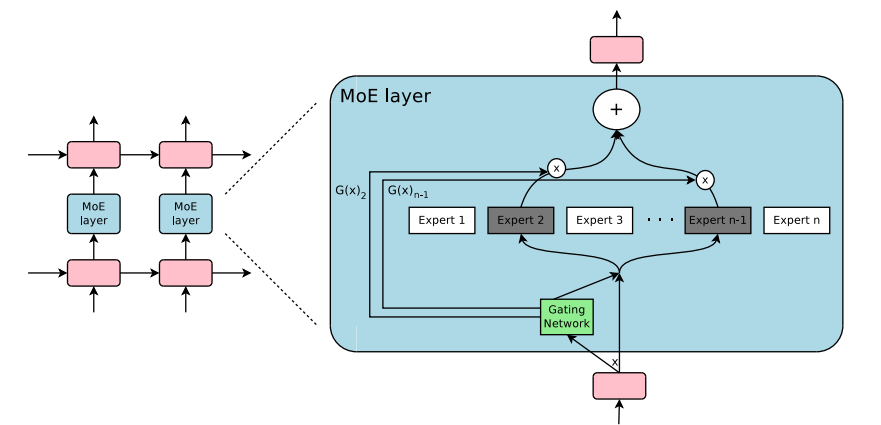
\includegraphics[width=\linewidth,height=0.52\textheight,keepaspectratio]{MoEArch.png}
    \caption{MoE layer: a router selects top-k experts for each token.}
\end{figure}
The key trade-off is that \underline{capacity depends on total parameters while inference speed depends on active parameters}: only top-$k$ experts run per token, so per-token FLOPs stay comparable to a dense FFN while total parameters grow $\sim N\times$.
For example, DeepSeek-V4-Flash uses 256 routed experts with top-6 active, hidden size 4096, and per-expert intermediate 2048.

\subsection{Noise \& Load Balance}
The output is a weighted sum of the selected experts:
\[ y = \sum_{i=1}^{N} G(x)_i\, E_i(x) \]
where the gating $G(x)$ is a softmax over the top-$k$ raw scores:
\[ G(x) = \mathrm{Softmax}\big(\mathrm{KeepTopK}(H(x), k)\big) \]
and the raw scores $H(x)$ add a tunable Gaussian noise term used for load balancing during training:
\[ H(x)_i = (x\, W_g)_i + \mathrm{StandardNormal}() \cdot \mathrm{Softplus}\big((x\, W_{noise})_i\big) \]
Here $\mathrm{KeepTopK}(v, k)$ keeps the top-$k$ entries of $v$ and sets the rest to $-\infty$, so the softmax concentrates all mass on the selected experts.
The weights $g_i = G(x)_i$ are dynamic activations computed per token, while only $W_g$ and $W_{noise}$ are static parameters.
Softmax is one gating choice; DeepSeek instead uses sigmoid scores with re-normalization.

\section{GShard}
Obviously, since tokens are dispatched to experts, the expert demension has \underline{naturally parallelism}. GShard scales MoE with expert parallelism plus all-to-all dispatch/combine, where all-to-all is a whole-cluster operation (the entire cluster is one group) rather than a per-node exchange. The round trip per MoE layer is:
\begin{enumerate}
    \item \textbf{Sharding}: the input $[B, L, E]$ is sharded along the token dimension; the layout starts uniform/balanced.
    \item \textbf{Router + All2All dispatch}: each device gates its local tokens, then dispatches each token to the device holding its assigned experts; the distribution becomes unbalanced (skewed).
    \item \textbf{Expert + All2All combine}: each device runs its own experts, then combine sends results back and performs the weighted sum; the layout returns to the original balanced one.
\end{enumerate}

\underline{About the Notations}: Usually $[B, L, E]$ are used in training, but only $[M, E]$ in trainning, sometimes $B$ can be seen as number of request.

\begin{figure}[!ht]
    \centering
    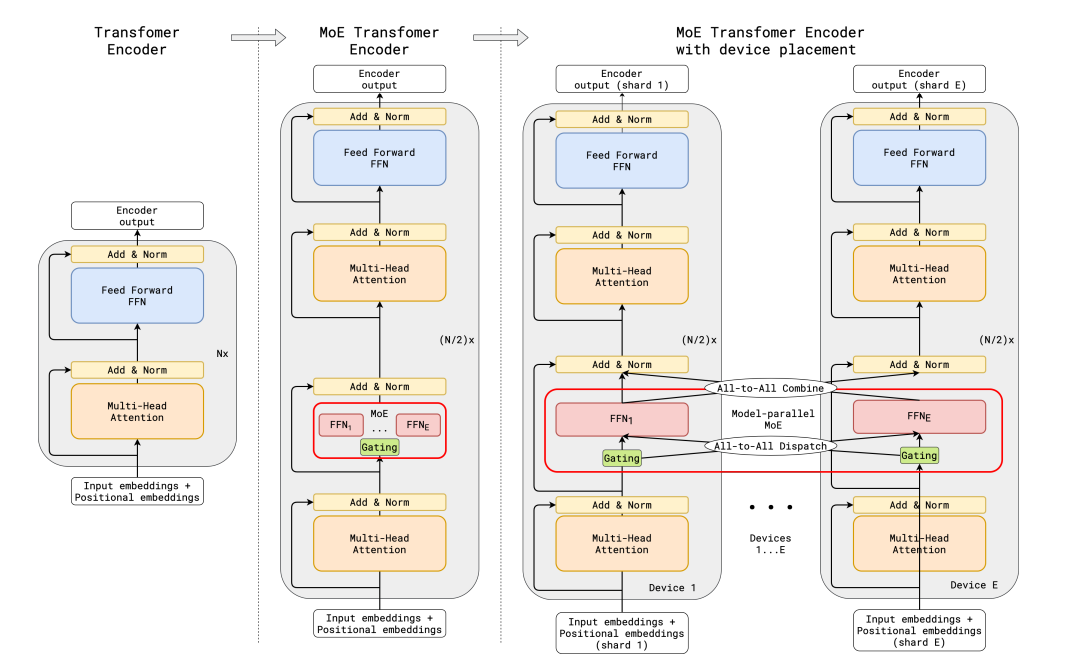
\includegraphics[width=\linewidth,height=0.52\textheight,keepaspectratio]{GshardArch.png}
    \caption{GShard: token sharding, dispatch (all-to-all), expert compute, combine (all-to-all).}
\end{figure}

\section{Implementation}
\textcolor{red}{TODO: Learn SGLang and weight loading}

\begin{thebibliography}{1}
    \bibitem{hf-moe}
    O. Sanseviero et al., \emph{Mixture of Experts Explained}, Hugging Face Blog, 2023, \href{https://huggingface.co/blog/moe}{huggingface.co/blog/moe}.
    \bibitem{hf-moe-transformers}
    A. R. Gosthipaty et al., \emph{Mixture of Experts (MoEs) in Transformers}, Hugging Face Blog, 2026, \href{https://huggingface.co/blog/moe-transformers}{huggingface.co/blog/moe-transformers}.
    \bibitem{gshard}
    D. Lepikhin et al., \emph{GShard: Scaling Giant Models with Conditional Computation and Automatic Sharding}, 2020, \href{https://arxiv.org/abs/2006.16668}{arXiv:2006.16668}.
\end{thebibliography}

\end{document}
